\documentclass[]{article}
\usepackage{lmodern}
\usepackage{amssymb,amsmath}
\usepackage{ifxetex,ifluatex}
\usepackage{fixltx2e} % provides \textsubscript
\ifnum 0\ifxetex 1\fi\ifluatex 1\fi=0 % if pdftex
  \usepackage[T1]{fontenc}
  \usepackage[utf8]{inputenc}
\else % if luatex or xelatex
  \ifxetex
    \usepackage{mathspec}
  \else
    \usepackage{fontspec}
  \fi
  \defaultfontfeatures{Ligatures=TeX,Scale=MatchLowercase}
\fi
% use upquote if available, for straight quotes in verbatim environments
\IfFileExists{upquote.sty}{\usepackage{upquote}}{}
% use microtype if available
\IfFileExists{microtype.sty}{%
\usepackage{microtype}
\UseMicrotypeSet[protrusion]{basicmath} % disable protrusion for tt fonts
}{}
\usepackage[margin=1in]{geometry}
\usepackage{hyperref}
\hypersetup{unicode=true,
            pdftitle={Assessed Problem Sheet 1},
            pdfauthor={Dom Hutchinson},
            pdfborder={0 0 0},
            breaklinks=true}
\urlstyle{same}  % don't use monospace font for urls
\usepackage{color}
\usepackage{fancyvrb}
\newcommand{\VerbBar}{|}
\newcommand{\VERB}{\Verb[commandchars=\\\{\}]}
\DefineVerbatimEnvironment{Highlighting}{Verbatim}{commandchars=\\\{\}}
% Add ',fontsize=\small' for more characters per line
\usepackage{framed}
\definecolor{shadecolor}{RGB}{248,248,248}
\newenvironment{Shaded}{\begin{snugshade}}{\end{snugshade}}
\newcommand{\AlertTok}[1]{\textcolor[rgb]{0.94,0.16,0.16}{#1}}
\newcommand{\AnnotationTok}[1]{\textcolor[rgb]{0.56,0.35,0.01}{\textbf{\textit{#1}}}}
\newcommand{\AttributeTok}[1]{\textcolor[rgb]{0.77,0.63,0.00}{#1}}
\newcommand{\BaseNTok}[1]{\textcolor[rgb]{0.00,0.00,0.81}{#1}}
\newcommand{\BuiltInTok}[1]{#1}
\newcommand{\CharTok}[1]{\textcolor[rgb]{0.31,0.60,0.02}{#1}}
\newcommand{\CommentTok}[1]{\textcolor[rgb]{0.56,0.35,0.01}{\textit{#1}}}
\newcommand{\CommentVarTok}[1]{\textcolor[rgb]{0.56,0.35,0.01}{\textbf{\textit{#1}}}}
\newcommand{\ConstantTok}[1]{\textcolor[rgb]{0.00,0.00,0.00}{#1}}
\newcommand{\ControlFlowTok}[1]{\textcolor[rgb]{0.13,0.29,0.53}{\textbf{#1}}}
\newcommand{\DataTypeTok}[1]{\textcolor[rgb]{0.13,0.29,0.53}{#1}}
\newcommand{\DecValTok}[1]{\textcolor[rgb]{0.00,0.00,0.81}{#1}}
\newcommand{\DocumentationTok}[1]{\textcolor[rgb]{0.56,0.35,0.01}{\textbf{\textit{#1}}}}
\newcommand{\ErrorTok}[1]{\textcolor[rgb]{0.64,0.00,0.00}{\textbf{#1}}}
\newcommand{\ExtensionTok}[1]{#1}
\newcommand{\FloatTok}[1]{\textcolor[rgb]{0.00,0.00,0.81}{#1}}
\newcommand{\FunctionTok}[1]{\textcolor[rgb]{0.00,0.00,0.00}{#1}}
\newcommand{\ImportTok}[1]{#1}
\newcommand{\InformationTok}[1]{\textcolor[rgb]{0.56,0.35,0.01}{\textbf{\textit{#1}}}}
\newcommand{\KeywordTok}[1]{\textcolor[rgb]{0.13,0.29,0.53}{\textbf{#1}}}
\newcommand{\NormalTok}[1]{#1}
\newcommand{\OperatorTok}[1]{\textcolor[rgb]{0.81,0.36,0.00}{\textbf{#1}}}
\newcommand{\OtherTok}[1]{\textcolor[rgb]{0.56,0.35,0.01}{#1}}
\newcommand{\PreprocessorTok}[1]{\textcolor[rgb]{0.56,0.35,0.01}{\textit{#1}}}
\newcommand{\RegionMarkerTok}[1]{#1}
\newcommand{\SpecialCharTok}[1]{\textcolor[rgb]{0.00,0.00,0.00}{#1}}
\newcommand{\SpecialStringTok}[1]{\textcolor[rgb]{0.31,0.60,0.02}{#1}}
\newcommand{\StringTok}[1]{\textcolor[rgb]{0.31,0.60,0.02}{#1}}
\newcommand{\VariableTok}[1]{\textcolor[rgb]{0.00,0.00,0.00}{#1}}
\newcommand{\VerbatimStringTok}[1]{\textcolor[rgb]{0.31,0.60,0.02}{#1}}
\newcommand{\WarningTok}[1]{\textcolor[rgb]{0.56,0.35,0.01}{\textbf{\textit{#1}}}}
\usepackage{graphicx,grffile}
\makeatletter
\def\maxwidth{\ifdim\Gin@nat@width>\linewidth\linewidth\else\Gin@nat@width\fi}
\def\maxheight{\ifdim\Gin@nat@height>\textheight\textheight\else\Gin@nat@height\fi}
\makeatother
% Scale images if necessary, so that they will not overflow the page
% margins by default, and it is still possible to overwrite the defaults
% using explicit options in \includegraphics[width, height, ...]{}
\setkeys{Gin}{width=\maxwidth,height=\maxheight,keepaspectratio}
\IfFileExists{parskip.sty}{%
\usepackage{parskip}
}{% else
\setlength{\parindent}{0pt}
\setlength{\parskip}{6pt plus 2pt minus 1pt}
}
\setlength{\emergencystretch}{3em}  % prevent overfull lines
\providecommand{\tightlist}{%
  \setlength{\itemsep}{0pt}\setlength{\parskip}{0pt}}
\setcounter{secnumdepth}{0}
% Redefines (sub)paragraphs to behave more like sections
\ifx\paragraph\undefined\else
\let\oldparagraph\paragraph
\renewcommand{\paragraph}[1]{\oldparagraph{#1}\mbox{}}
\fi
\ifx\subparagraph\undefined\else
\let\oldsubparagraph\subparagraph
\renewcommand{\subparagraph}[1]{\oldsubparagraph{#1}\mbox{}}
\fi

%%% Use protect on footnotes to avoid problems with footnotes in titles
\let\rmarkdownfootnote\footnote%
\def\footnote{\protect\rmarkdownfootnote}

%%% Change title format to be more compact
\usepackage{titling}

% Create subtitle command for use in maketitle
\providecommand{\subtitle}[1]{
  \posttitle{
    \begin{center}\large#1\end{center}
    }
}

\setlength{\droptitle}{-2em}

  \title{Assessed Problem Sheet 1}
    \pretitle{\vspace{\droptitle}\centering\huge}
  \posttitle{\par}
  \subtitle{Statistics 1}
  \author{Dom Hutchinson}
    \preauthor{\centering\large\emph}
  \postauthor{\par}
    \date{}
    \predate{}\postdate{}
  

\begin{document}
\maketitle

\begin{Shaded}
\begin{Highlighting}[]
\KeywordTok{load}\NormalTok{(}\KeywordTok{url}\NormalTok{(}\StringTok{"https://people.maths.bris.ac.uk/~maxca/stats1/stats1-assignment.RData"}\NormalTok{))}
\end{Highlighting}
\end{Shaded}

\hypertarget{question-4}{%
\section{Question 4}\label{question-4}}

\begin{Shaded}
\begin{Highlighting}[]
\NormalTok{compute.ad.test <-}\StringTok{ }\ControlFlowTok{function}\NormalTok{ (xs) \{}
\NormalTok{  len<-}\KeywordTok{length}\NormalTok{(xs)  }\CommentTok{# Length of vector}
\NormalTok{  sorted<-}\KeywordTok{sort}\NormalTok{(xs) }\CommentTok{# Sort vector}
  
\NormalTok{  xBar<-}\KeywordTok{mean}\NormalTok{(xs)   }\CommentTok{# Sample mean}
\NormalTok{  S<-}\KeywordTok{sd}\NormalTok{(xs)        }\CommentTok{# Sample standard deviation}
  
\NormalTok{  summation<-}\DecValTok{0}
  \ControlFlowTok{for}\NormalTok{ (j }\ControlFlowTok{in} \DecValTok{1}\OperatorTok{:}\NormalTok{len) \{                             }\CommentTok{# Calculate each element of summation}
\NormalTok{    scalar<-(}\DecValTok{2}\OperatorTok{*}\NormalTok{j}\DecValTok{-1}\NormalTok{)}\OperatorTok{/}\NormalTok{len                          }\CommentTok{# Scalar of element}
\NormalTok{    first<-}\KeywordTok{log}\NormalTok{(}\KeywordTok{pnorm}\NormalTok{(sorted[j],xBar,S))          }\CommentTok{# First ln term}
\NormalTok{    second<-}\KeywordTok{log}\NormalTok{(}\DecValTok{1}\OperatorTok{-}\KeywordTok{pnorm}\NormalTok{(sorted[len}\OperatorTok{+}\DecValTok{1}\OperatorTok{-}\NormalTok{j],xBar,S)) }\CommentTok{# Second ln term}
\NormalTok{    element<-scalar}\OperatorTok{*}\NormalTok{(first}\OperatorTok{+}\NormalTok{second)               }\CommentTok{# Value of j^th of summation}
\NormalTok{    summation<-summation}\OperatorTok{+}\NormalTok{element                 }\CommentTok{# Add to summation}
\NormalTok{  \}}
  
\NormalTok{  T<-}\OperatorTok{-}\KeywordTok{length}\NormalTok{(xs)}\OperatorTok{-}\NormalTok{summation }\CommentTok{# Test statistic }
  \KeywordTok{return}\NormalTok{ (T)}
\NormalTok{\}}
\KeywordTok{compute.ad.test}\NormalTok{(x1)}
\end{Highlighting}
\end{Shaded}

\begin{verbatim}
## [1] 0.4369709
\end{verbatim}

\begin{Shaded}
\begin{Highlighting}[]
\KeywordTok{compute.ad.test}\NormalTok{(x2)}
\end{Highlighting}
\end{Shaded}

\begin{verbatim}
## [1] 0.8406134
\end{verbatim}

\hypertarget{question-6}{%
\section{Question 6}\label{question-6}}

\begin{Shaded}
\begin{Highlighting}[]
\NormalTok{compute.ad.pvalue <-}\StringTok{ }\ControlFlowTok{function}\NormalTok{ (xs) \{}
\NormalTok{  sampleSize=}\DecValTok{10}  \CommentTok{# Size of each sample}
\NormalTok{  numSamples=}\DecValTok{500} \CommentTok{# Number of samples}
  
\NormalTok{  xBar<-}\KeywordTok{mean}\NormalTok{(xs)             }\CommentTok{# Sample mean}
\NormalTok{  s<-}\KeywordTok{sd}\NormalTok{(xs)                  }\CommentTok{# Sample standard deviation}
\NormalTok{  t_obs<-}\KeywordTok{compute.ad.test}\NormalTok{(xs) }\CommentTok{# Observed Statistic}
  
\NormalTok{  gvalues<-}\KeywordTok{rnorm}\NormalTok{(sampleSize}\OperatorTok{*}\NormalTok{numSamples,xBar,s)        }\CommentTok{# Generate values from N(xBar,s)}
\NormalTok{  gsamples<-}\KeywordTok{matrix}\NormalTok{(gvalues,}\DataTypeTok{nrow=}\NormalTok{numSamples)           }\CommentTok{# Group into samples}
\NormalTok{  gsamples.ad.test<-}\KeywordTok{apply}\NormalTok{(gsamples,}\DecValTok{1}\NormalTok{,compute.ad.test) }\CommentTok{# Calcualate AD statistic for each sample}
  
\NormalTok{  num=}\KeywordTok{sum}\NormalTok{(gsamples.ad.test}\OperatorTok{>=}\NormalTok{t_obs) }\CommentTok{# Number of simulated statistics >= given}
\NormalTok{  p=num}\OperatorTok{/}\NormalTok{numSamples                 }\CommentTok{# As proportion}
  
  \CommentTok{# Create plots}
  \KeywordTok{par}\NormalTok{(}\DataTypeTok{mfrow=}\KeywordTok{c}\NormalTok{(}\DecValTok{1}\NormalTok{,}\DecValTok{2}\NormalTok{))}
  \KeywordTok{hist}\NormalTok{(gsamples.ad.test,}\DataTypeTok{main=}\StringTok{"Histogram of Simulated Statistics"}\NormalTok{)}
  \KeywordTok{abline}\NormalTok{(}\DataTypeTok{v=}\NormalTok{t_obs,}\DataTypeTok{col=}\StringTok{"red"}\NormalTok{)}
  \KeywordTok{qqnorm}\NormalTok{(gsamples.ad.test)}
  \KeywordTok{qqline}\NormalTok{(gsamples.ad.test)}
  
  \KeywordTok{return}\NormalTok{ (p)}
\NormalTok{\}}

\KeywordTok{compute.ad.pvalue}\NormalTok{(x1)}
\end{Highlighting}
\end{Shaded}

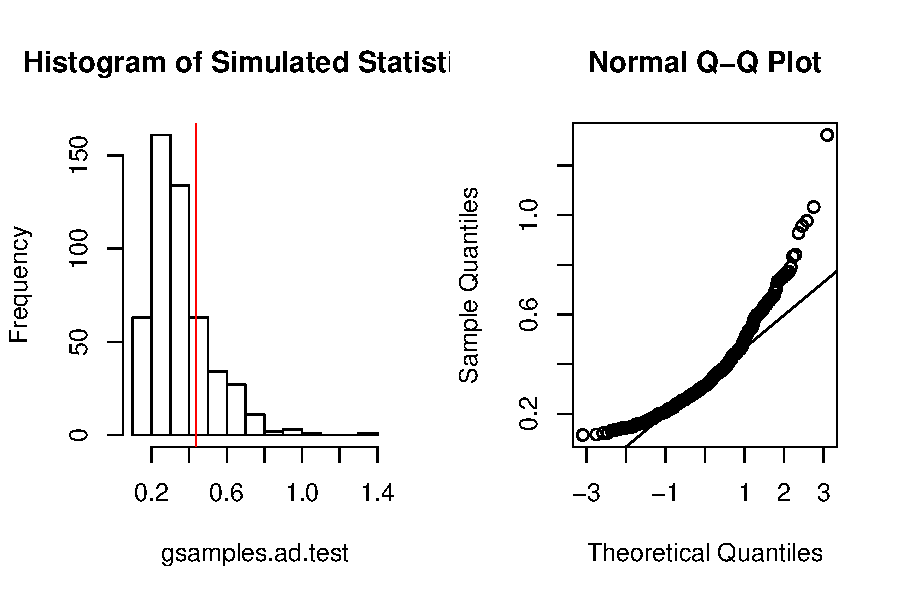
\includegraphics{Assessed1S1_files/figure-latex/unnamed-chunk-3-1.pdf}

\begin{verbatim}
## [1] 0.234
\end{verbatim}

\begin{Shaded}
\begin{Highlighting}[]
\KeywordTok{compute.ad.pvalue}\NormalTok{(x2)}
\end{Highlighting}
\end{Shaded}

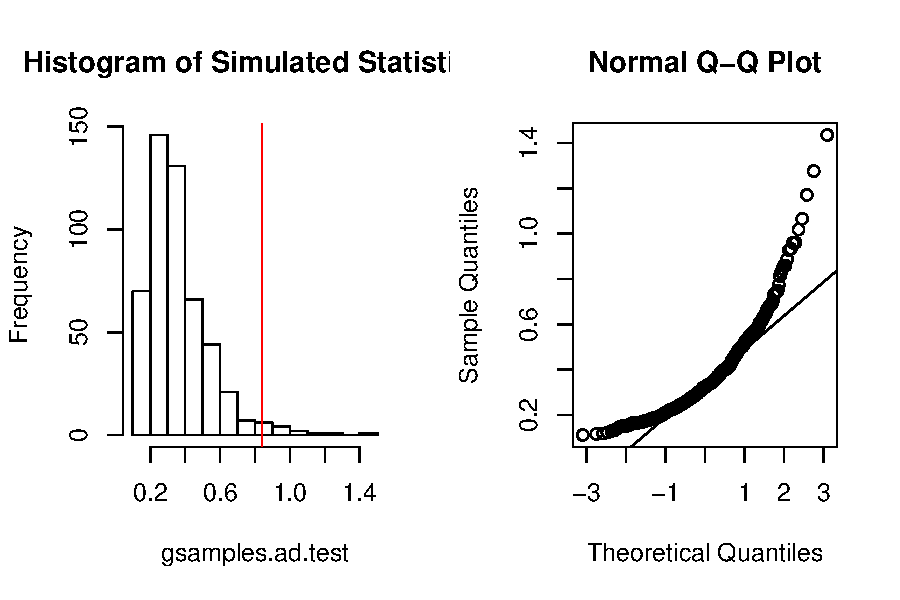
\includegraphics{Assessed1S1_files/figure-latex/unnamed-chunk-3-2.pdf}

\begin{verbatim}
## [1] 0.026
\end{verbatim}


\end{document}
